\section{ReTrace}
\label{sec:method}

ReTrace must reproduce at verification time every decision that determines which tokens
are scored. This requirement divides the method into four modules. The
\emph{Reproducible Response Bank} (RRB) records how the DLM responds to a fixed family of
context ablations (\S\ref{sec:observable}). The \emph{Balanced Carrier Gate} (BCG) admits
only positions with usable probability mass on both response signs. The
\emph{Response-Aligned Resampler} (RAR) embeds evidence without changing the reference
block schedule (\S\ref{sec:embedding}), and the \emph{Response-Replay Verifier} (RRV)
reconstructs the RRB from the completed text and applies an exact test
(\S\ref{sec:theory}).

\subsection{Reproducible Response Bank}
\label{sec:observable}

Consider a block $B_b$ beginning at position $r_b$. Let $F_b$ contain the prompt and all
positions before $B_b$, which are final when the block starts. ReTrace constructs $L$
equal-size ablation patterns $D_{b,1},\ldots,D_{b,L}\subset F_b$. The implementation
includes near-context, far-context, and keyed pseudorandom patterns. For pattern $\ell$,
the model input masks $D_{b,\ell}$, the entire current block, and every later block. For
each $i\in B_b$ and vocabulary item $v$, one masked sequence evaluation yields
\begin{equation}
\ell_{i,\ell}(v)
  = \log p_\theta\!\left(v \mid F_b\setminus D_{b,\ell};
                    B_b\text{ and suffix masked}\right).
\label{eq:arm-logprob}
\end{equation}

Masking the current block is essential. It prevents tokens committed later in that block
from changing the RRB. Masking the suffix is equally important because those tokens were
not visible when the embedder built the bank. Given the completed text, the RRV restores
exactly this state by re-masking the current block and suffix. Thus the RRB depends on the
final prefix, model, public parameters, and key, but not on an unrecorded generation
trajectory.

For an unordered pair of patterns $(u,v)$, define
\begin{equation}
g_i^{u,v}(z)=\ell_{i,v}(z)-\ell_{i,u}(z).
\label{eq:g}
\end{equation}
Let $p_i^{\mathrm{base}}$ denote the model distribution when $B_b$ and the suffix are
masked but no context pattern is ablated. The probability mass on each sign is
\begin{equation}
q_{i,+}^{u,v}=\sum_z p_i^{\mathrm{base}}(z)
                  \mathbf{1}[g_i^{u,v}(z)>0],\qquad
q_{i,-}^{u,v}=\sum_z p_i^{\mathrm{base}}(z)
                  \mathbf{1}[g_i^{u,v}(z)<0],
\label{eq:sign-mass}
\end{equation}
and the two-sided score is
\begin{equation}
S_i^{u,v}=2\min(q_{i,+}^{u,v},q_{i,-}^{u,v}).
\label{eq:gate}
\end{equation}
ReTrace chooses, independently at each position, the pair with the largest $S_i^{u,v}$
and stores its contrast as $g_i$ in the RRB. The \emph{Balanced Carrier Gate} then admits
position $i$ when $S_i>s_{\min}$; an optional per-block cap retains the largest scores.
Because $S_i^{u,v}$ is unchanged when $u$ and $v$ are swapped, the BCG neither observes nor
favors the requested orientation. Both pair selection and gating are recomputable from the
block-masked state.

\subsection{Response-Replay Verifier and exact null}
\label{sec:theory}

The key derives an orientation $\epsilon_i\in\{-1,+1\}$ for every position using a PRF
domain separate from pattern generation, pair selection, carrier assignment, and payload
grouping. A target $w_i\in\{-1,+1\}$ represents the desired provenance or message bit.
For a nonzero contrast, position $i$ matches when
\begin{equation}
m_i=\mathbf{1}[w_i\epsilon_i g_i(y_i)>0].
\label{eq:m}
\end{equation}
If $g_i(y_i)=0$ exactly, ReTrace uses an additional domain-separated fair tie bit for
$m_i$. Ties cannot be steered during embedding, but assigning all of them zero would bias
the null.

For provenance-only detection, all carriers form a presence pool $P$ with $w_i=+1$. If a
payload is enabled, the implementation can reserve a synchronization subset for presence
and partition the remaining carriers by payload bit. These groups must remain separate:
aggregating a balanced message would cancel positive and negative targets. The presence
statistic and its one-sided $p$-value are
\begin{equation}
T=\sum_{i\in P}m_i,\qquad
p_{\mathrm{det}}=\Pr\!\left[\mathrm{Binomial}(|P|,\tfrac12)\geq T\right].
\label{eq:test}
\end{equation}

\begin{proposition}[Conditional exact null]
\label{prop:null}
Assume the PRF domains above behave as independent random functions. Fix any text $y$
generated independently of the document key, and condition on the carrier set, selected
pairs, contrast values, payload roles, and target bits. The orientation bits (and tie bits
where needed) remain independent fair coins. Consequently, the $m_i$ are independent
$\mathrm{Bernoulli}(\tfrac12)$ variables and
$T\sim\mathrm{Binomial}(|P|,\tfrac12)$ exactly.
\end{proposition}

The proposition is conditional on the observed text and therefore requires neither a text
distribution nor an asymptotic approximation. Its guarantee does rely on correct domain
separation and on the text being independent of the document key under the null. The
implementation enforces this separation with distinct HMAC labels.

\subsection{Response-Aligned Resampling}
\label{sec:embedding}

\begin{algorithm}[H]
\caption{\textbf{ReTrace embedding and verification.} \textsc{Build-RRB} is shared
verbatim by the RAR and RRV. The reference block order, confidence selection, and live DLM
conditional are unchanged; guided retries reuse the current probability row.}
\label{alg:retrace}
\small
\textbf{Input:} prompt $x_{<B_1}$, key $K$, retry budget $R$, floor $\kappa$,
threshold $s_{\min}$ \qquad \textbf{Output:} generated text $y$ or $p_{\rm det}$
\vspace{2pt}

\begin{tabular}{@{}r@{\hspace{0.65em}}p{0.91\linewidth}@{}}
\multicolumn{2}{@{}l}{\textsc{Build-RRB}$(x,b,K)$ --- Reproducible Response Bank}\\
1 & Mask the current block $B_b$ and suffix; construct $L$ keyed ablations of the fixed prefix.\\
2 & Evaluate the $L$ ablated sequences and one unablated sequence with the DLM.\\
3 & For every $i\in B_b$, select $(u,v)=\arg\max_{u<v}S_i^{u,v}$ and store
    $g_i=\ell_{i,v}-\ell_{i,u}$ and $S_i=2\min(q_{i,+},q_{i,-})$.\\[2pt]
\multicolumn{2}{@{}l}{\textsc{Embed}$(x,K,R,\kappa)$ --- Response-Aligned Resampler}\\
4 & \textbf{for} each block $B_b$ in reference order \textbf{do}; compute
    $\mathcal{R}_b\leftarrow\textsc{Build-RRB}(x,b,K)$.\\
5 & \quad\textbf{while} $B_b$ contains masks \textbf{do}; let the reference confidence
    rule select positions and obtain each live row $p_i$.\\
6 & \qquad\textbf{if} $S_i\leq s_{\min}$, draw $z\sim p_i$ once.\\
7 & \qquad\textbf{else} draw at most $R$ proposals from $p_i$; accept the first
    $z$ satisfying $w_i\epsilon_i g_i(z)>0$ and $p_i(z)\geq\kappa\max_v p_i(v)$.\\
8 & \qquad\textbf{if} no guided proposal is accepted, draw one fresh unchecked
    $z\sim p_i$; commit $z$.\\[2pt]
\multicolumn{2}{@{}l}{\textsc{Verify}$(y,K)$ --- Response-Replay Verifier}\\
9 & Re-mask each completed block and suffix; rebuild $\mathcal{R}_b$ with
    \textsc{Build-RRB}$(y,b,K)$.\\
10 & Apply the BCG, compute $m_i$ at admitted carriers, and return the exact binomial tail
     in Eq.~\eqref{eq:test}.\\
\end{tabular}
\end{algorithm}

Algorithm~\ref{alg:retrace} makes the module boundaries explicit. Within each block, the
RAR uses the reference confidence order and live conditional $p_i$. Positions rejected by
the BCG are sampled normally. At an admitted carrier, define the acceptance set
\begin{equation}
A_i=\left\{z:
 w_i\epsilon_i g_i(z)>0\ \text{ and }\
 p_i(z)\geq \kappa\max_v p_i(v)
\right\}.
\label{eq:accept-set}
\end{equation}
The RAR draws independently from $p_i$ up to $R$ times and commits the first proposal
in $A_i$. If none is accepted, it makes one fresh unconditional draw from $p_i$ and commits
it without inspection. The probability row does not change during these retries, so they
do not require additional model evaluations.

This procedure changes the sampling distribution. Let
$a_i=p_i(A_i)$ be the acceptance mass and let
\begin{equation}
q_i=\sum_z p_i(z)m_i(z)
\label{eq:q-live}
\end{equation}
where $m_i(z)$ applies Eq.~\eqref{eq:m} and the tie rule to candidate $z$. Thus $q_i$ is
the probability that an unconditional draw is scored as a detector hit, irrespective of
the plausibility floor. The committed-token distribution is
\begin{equation}
\left(1-(1-a_i)^R\right)p_i(\cdot\mid A_i)
 +(1-a_i)^R p_i,
\label{eq:dist}
\end{equation}
and its detector-hit probability is
\begin{equation}
\Pr[m_i=1]=1-(1-a_i)^R(1-q_i).
\label{eq:hit}
\end{equation}
When $\kappa=0$ and the conditional assigns no mass to exact ties, $a_i=q_i$ and
Eq.~\eqref{eq:hit} reduces to $1-(1-q_i)^{R+1}$. Separating $a_i$ and $q_i$ is necessary
when the plausibility floor or tie rule is active: a fallback token may score as a hit even
if it could not have been accepted as a guided proposal.

The floor bounds the model NLL of every \emph{guided accepted} proposal to within
$-\log\kappa$ of the live argmax. It does not guarantee better semantic quality, and the
unconditional fallback remains unrestricted. Similarly, saying that every output was
proposed by the model is a support statement, not a distortion-free claim. Equation
\eqref{eq:dist} makes the distributional change explicit.

\begin{figure}[t]
\centering
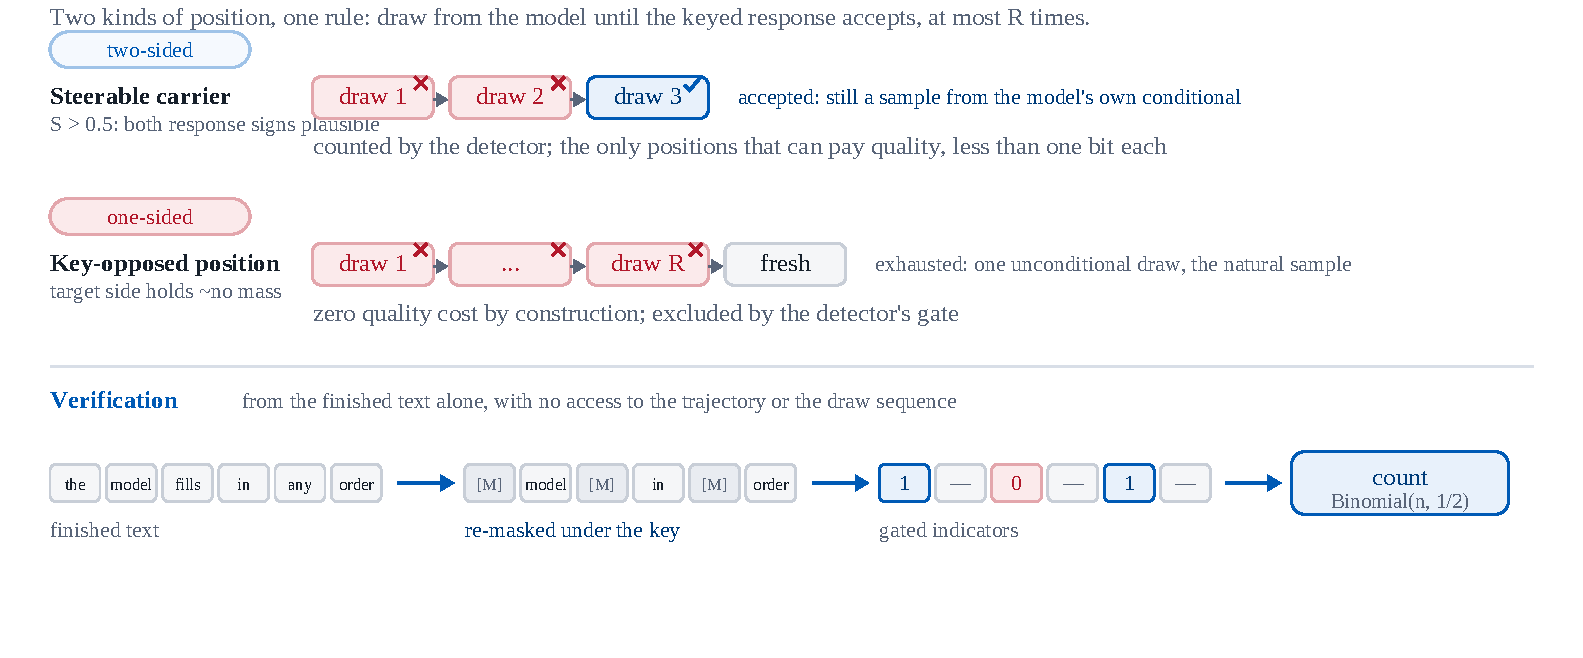
\includegraphics[width=\linewidth]{figures/fig_retrace_mechanism.pdf}
\caption{\textbf{The Balanced Carrier Gate separates usable response channels from
orientation-dependent ones.} The BCG admits a position only when both signs carry
substantial mass under the RRB's block-masked conditional. Its score is invariant to
swapping the response arms and is computed without consulting the keyed orientation.
Admitted positions are steered by the RAR and counted by the RRV; rejected positions follow
the reference sampler and contribute no detector trial.}
\label{fig:mechanism}
\end{figure}

The score $S_i$ is computed under the reproducible block-masked distribution, whereas
generation samples from the evolving live conditional. It is therefore a symmetric proxy
for live acceptance mass, not a guarantee that each carrier is easy to steer. Selecting
the best pair per position increases the measured mean two-sided score from $0.28$ for a
fixed near/far pair to $0.45$. This gate, the unconditional fallback, and the plausibility
floor are the three safeguards that determine ReTrace's empirical trade-off.

\subsection{Why not substitute tokens after generation?}
\label{sec:v1}

An earlier design first generated an unwatermarked text and then replaced selected tokens
with alternatives having the desired contrast sign. A candidate $z$ was admissible only if
its probability relative to the most likely token satisfied
$p(z)/p(z^\star)\geq e^{-\tau}$. This approach is simple and uses the same detector, but
the experiments show that it has too little capacity on the evaluated model.

Across 36 settings covering three carrier rules, three fluency budgets, and two guidance
weights, the median selected position had only one admissible token at $\tau=3$
($p(z)/p(z^\star)\geq0.05$). The best setting within a $1.35\times$ perplexity budget
reached only $0.10$ TPR at $1\%$ FPR, compared with $0.86$ for the local dgMARK
reproduction at $1.23\times$.

A sampler correction made the limitation clearer. Confidence had initially been computed
from Gumbel-perturbed logits rather than the clean model distribution. Fixing this error
reduced draft perplexity from $22.2$ to $9.5$ and mean conditional entropy from $0.655$ to
$0.319$. At the same time, the mean number of admissible alternatives fell from $2.5$ to
$1.6$ at $\tau=3$ and from $14.1$ to $5.6$ at $\tau=6$. In this setting, sharper
conditionals improve the base sampler while removing the alternatives needed for post-hoc
substitution.

This result motivates resampling rather than a universal claim that substitution must fail
for every DLM. ReTrace makes its choice while the model is already sampling and falls back
to an unconditional proposal when steering fails; it does not force a replacement after
the surrounding text has been fixed.

